\documentclass[french]{beamer}

\usepackage[utf8]{inputenc}
\usepackage[T1]{fontenc}
\usepackage{lmodern}
\usepackage{babel}
\usepackage{tikz}
\usepackage{graphicx}
\usetikzlibrary{arrows}

\usetheme{PaloAlto}

\tikzset{
  treenode/.style = {align=center, inner sep=0pt, text centered,
    font=\sffamily},
  arn_equi/.style = {treenode, circle, white, draw=green, fill=green, text width=1em},
  arn_notequi/.style = {treenode, circle, white, draw=red,fill=red, text width=1em},
  arn_new/.style = {treenode, circle, white, draw=blue,fill=blue, text width=1em},
  arn_null/.style = {treenode, rectangle, draw=black,minimum width=0.5em, minimum height=0.5em}
}



%Pour le TITLEPAGE
\title{CPROJ}
\subtitle{Rapport du Projet}
\author[]{MARINO Isabelle 21306227,  TIRICHINE Hafça 21307587,  JACQUETTE Pierrick 21305551}
\date{Avril 2016}
\institute[L3 S6-- Informatique]{Université Paris 7 Diderot}


\begin{document}

\begin{frame}
	\titlepage
\end{frame}

\begin{frame}
	\frametitle{Sommaire}
	\tableofcontents	
\end{frame}

\section{Librairies utilisées}
\begin{frame}{Librairies utilisées}
	\textbf{Pour parser les elements du document XML} :
	\begin{itemize}
	\item Libxml2
	\end{itemize}
	\textbf{Pour l'affichage graphique} :
	\begin{itemize}
	\item SDL2
	\item SDL2\_gfx 
	\end{itemize}
\end{frame}

\section{Graphe de structure}
\begin{frame}{Graphe de structure d'une Map}
	\begin{center}
	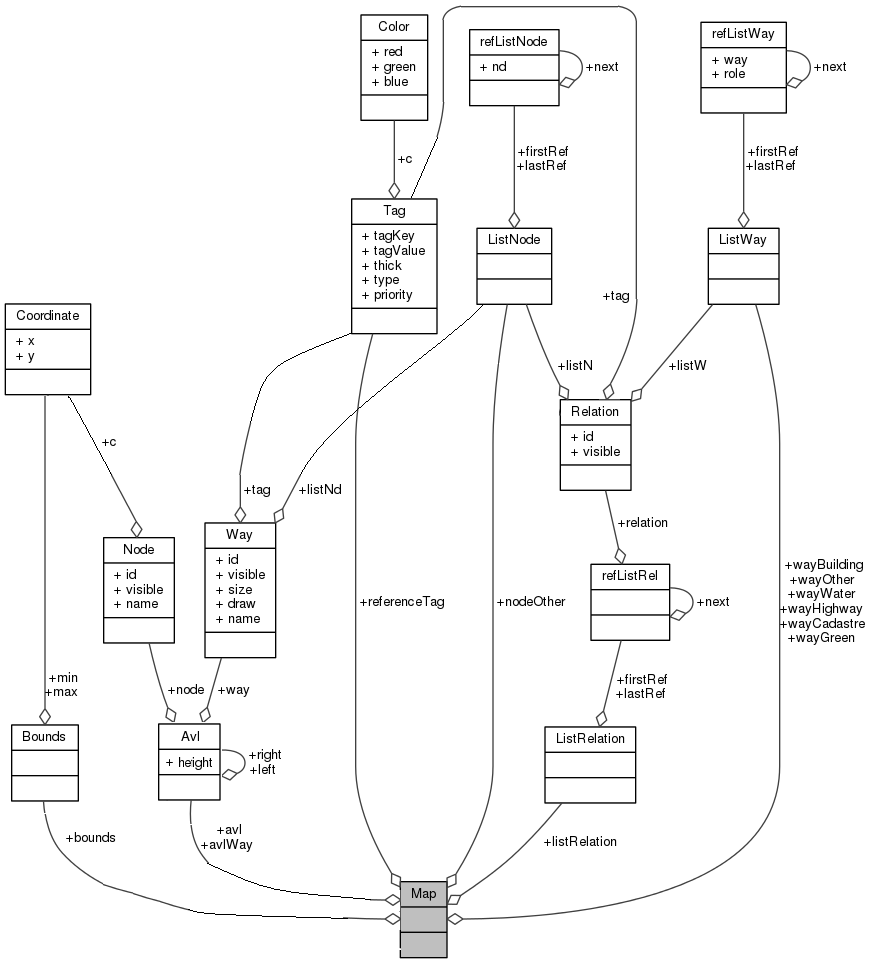
\includegraphics[width=6cm]{structures.png}
	\end{center}
\end{frame}

\section{AVL}
\begin{frame}{Stockage des Ways et des Nodes}
	\textbf{AVL} : C'est un ABR (arbre binaire de recherche) équilibré.
	On n'a pas besoin de conserver un ordre.
	\visible<2-3>{	
		Les opérations dont on a besoin (n est le nombre d'élément):
	}
	\begin{itemize}
	\item<2-3> \textbf{Insertion} : $\theta$(log n) : la hauteur de l'arbre
	\item<3>   \textbf{Recherche} : $\theta$(log n) : la hauteur de l'arbre
	\end{itemize}
\end{frame}

\begin{frame}[fragile]{Equilibrage lors d'une insertion}
\framesubtitle{Rotation simple gauche et droite}
	\begin{tabular}{ccc}
		 \multicolumn{2}{l}{
		 	\visible<1-4>{
	 			Diff de profondeur des ss-arbre de 2 et le FD une diff de 1.
	 		}
		 }
		 \\
	 	\visible<1-4>{		
			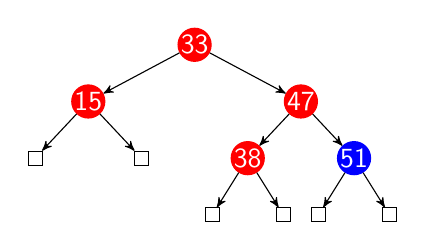
\begin{tikzpicture}[->,>=stealth',level/.style={sibling distance = 2.7cm/#1,level distance = 0.72cm}]
				\node [arn_notequi] {33}
		 				child{ node [arn_notequi] {15} 
		        			child{ node [arn_null] {}
						}
						child{ node [arn_null] {}
						}
		            	}                            
		    		    child{ node [arn_notequi] {47}
		            		child{ node [arn_notequi] {38} 
		            		    child{ node [arn_null] {}
							}
							child{ node [arn_null] {}
							}
		            		}
		            		child{ node [arn_new] {51}
		            		    child{ node [arn_null] {}
							}
							child{ node [arn_null] {}
							}
		            		}
					}
			; 
			\end{tikzpicture}
		}
		&
		\visible<2-4>{
			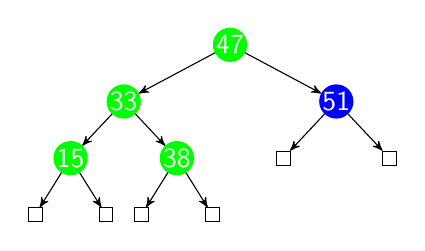
\begin{tikzpicture}[->,>=stealth',level/.style={sibling distance = 2.7cm/#1,level distance = 0.72cm}] 
				\node [arn_equi] {47}
	 				child{ node [arn_equi] {33} 
	        			child{ node [arn_equi] {15}
	    	         		child{ node [arn_null] {}
							}
							child{ node [arn_null] {}
							}       			 
	            		}                         
					  	child{ node [arn_equi] {38}
	    	         		child{ node [arn_null] {}
							}
							child{ node [arn_null] {}
							}  
						}
	            	}                            
	    		    child{ node [arn_new] {51}
	            		child{ node [arn_null] {}
						}
						child{ node [arn_null] {}
						}
	            	}			
			; 
			\end{tikzpicture}
		}
		\\
		\\
		\visible<3-4>{
			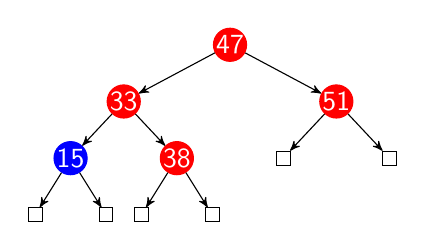
\begin{tikzpicture}[->,>=stealth',level/.style={sibling distance = 2.7cm/#1,level distance = 0.72cm}] 
				\node [arn_notequi] {47}
	 				child{ node [arn_notequi] {33} 
	        			child{ node [arn_new] {15}
	    	         		child{ node [arn_null] {}
							}
							child{ node [arn_null] {}
							}       			 
	            		}                         
					  	child{ node [arn_notequi] {38}
	    	         		child{ node [arn_null] {}
							}
							child{ node [arn_null] {}
							}  
						}
	            	}                            
	    		    child{ node [arn_notequi] {51}
	            		child{ node [arn_null] {}
						}
						child{ node [arn_null] {}
						}
	            	}			
			;  
			\end{tikzpicture}
		}
		&
		\visible<4>{
			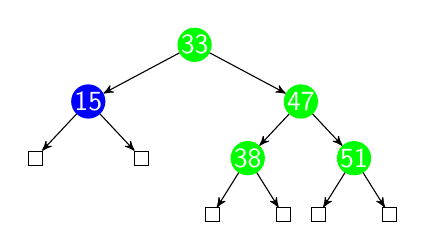
\begin{tikzpicture}[->,>=stealth',level/.style={sibling distance = 2.7cm/#1,level distance = 0.72cm}] 
				\node [arn_equi] {33}
	 				child{ node [arn_new] {15} 
	        			child{ node [arn_null] {}
						}
						child{ node [arn_null] {}
						}
	            	}                            
	    		    child{ node [arn_equi] {47}
	            		child{ node [arn_equi] {38} 
	            		    child{ node [arn_null] {}
							}
							child{ node [arn_null] {}
							}
	            		}
	            		child{ node [arn_equi] {51}
	            		    child{ node [arn_null] {}
							}
							child{ node [arn_null] {}
							}
	            		}
					}
			;
			\end{tikzpicture}
		}
		\\
		\multicolumn{2}{l}{
			\visible<3-4>{
				Diff de profondeur des ss-arbre de -2 et le FD une diff de -1.
			}
		}
		\\	
	\end{tabular}
\end{frame}

\begin{frame}[fragile]{Equilibrage lors d'une insertion}
\framesubtitle{Rotation double droite gauche et gauche droite}
	\begin{tabular}{ccc}
	 	\multicolumn{2}{l}{
	 		\visible<1-4>{
	 			Diff de profondeur des ss-arbre de 2 et le FD une diff de -1.
	 		}
	 	}
	 	\\
	 	\visible<1-4>{
			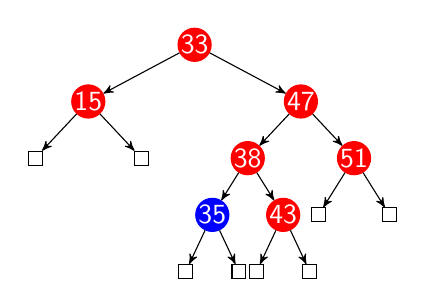
\begin{tikzpicture}[->,>=stealth',level/.style={sibling distance = 2.7cm/#1,level distance = 0.72cm}]
				\node [arn_notequi] {33}
	 				child{ node [arn_notequi] {15} 
	        			child{ node [arn_null] {}
						}
						child{ node [arn_null] {}
						}
	            	}                            
	    		    child{ node [arn_notequi] {47}
	            		child{ node [arn_notequi] {38}
	            			child{ node [arn_new] {35}
	            			    child{ node [arn_null] {}
								}
								child{ node [arn_null] {}
								}
							}
							child{ node [arn_notequi] {43}
							    child{ node [arn_null] {}
								}
								child{ node [arn_null] {}
								}
							}
	            		}
	            		child{ node [arn_notequi] {51}
	            		    child{ node [arn_null] {}
							}
							child{ node [arn_null] {}
							}
	            		}
					}
			; 
			\end{tikzpicture}
		}
		&
		\visible<2-4>{
			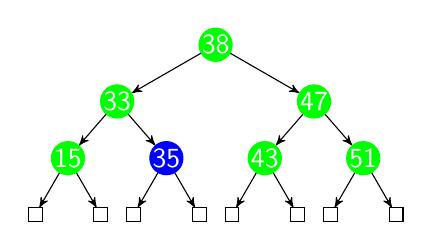
\begin{tikzpicture}[->,>=stealth',level/.style={sibling distance = 2.5cm/#1,level distance = 0.72cm}] 
				\node [arn_equi] {38}
	 				child{ node [arn_equi] {33} 
	        			child{ node [arn_equi] {15}
	    	         		child{ node [arn_null] {}
							}
							child{ node [arn_null] {}
							}       			 
	            		}                         
					  	child{ node [arn_new] {35}
	    	         		child{ node [arn_null] {}
							}
							child{ node [arn_null] {}
							}  
						}
	            	}                            
	    		    child{ node [arn_equi] {47}
	            		child{ node [arn_equi] {43}
	    	         		child{ node [arn_null] {}
							}
							child{ node [arn_null] {}
							}       			 
	            		}                         
					  	child{ node [arn_equi] {51}
	    	         		child{ node [arn_null] {}
							}
							child{ node [arn_null] {}
							}  
						}
	            	}			
			; 
			\end{tikzpicture}
		}
		\\
		\visible<3-4>{
			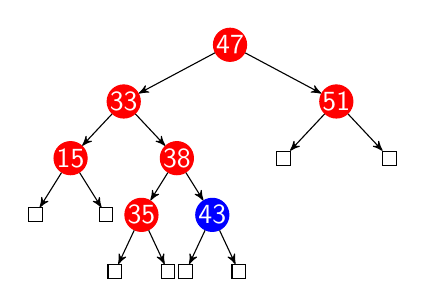
\begin{tikzpicture}[->,>=stealth',level/.style={sibling distance = 2.7cm/#1,level distance = 0.72cm}] 
				\node [arn_notequi] {47}
					child{ node [arn_notequi] {33}
	            		child{ node [arn_notequi] {15}
	            			child{ node [arn_null] {}
							}
							child{ node [arn_null] {}
							}
						}
			        	child{ node [arn_notequi] {38}
	            			child{ node [arn_notequi] {35}
	            			    child{ node [arn_null] {}
								}
								child{ node [arn_null] {}
								}
							}
							child{ node [arn_new] {43}
							    child{ node [arn_null] {}
								}
								child{ node [arn_null] {}
								}
							}
	            		}
					}
	 				child{ node [arn_notequi] {51} 
	        			child{ node [arn_null] {}
						}
						child{ node [arn_null] {}
						}
	            	}
			;  
			\end{tikzpicture} 
		}
		&
		\visible<4>{
			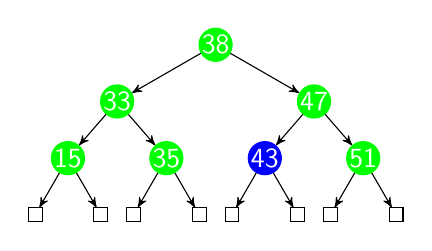
\begin{tikzpicture}[->,>=stealth',level/.style={sibling distance = 2.5cm/#1,level distance = 0.72cm}] 
				\node [arn_equi] {38}
	 				child{ node [arn_equi] {33} 
	        			child{ node [arn_equi] {15}
	    	         		child{ node [arn_null] {}
							}
							child{ node [arn_null] {}
							}       			 
	            		}                         
					  	child{ node [arn_equi] {35}
	    	         		child{ node [arn_null] {}
							}
							child{ node [arn_null] {}
							}  
						}
	            	}                            
	    		    child{ node [arn_equi] {47}
	            		child{ node [arn_new] {43}
	    	         		child{ node [arn_null] {}
							}
							child{ node [arn_null] {}
							}       			 
	            		}                         
					  	child{ node [arn_equi] {51}
	    	         		child{ node [arn_null] {}
							}
							child{ node [arn_null] {}
							}  
						}
	            	}			
			; 
			\end{tikzpicture}
		}
		\\
		 \multicolumn{2}{l}{
		 	\visible<4>{
		 		Diff de profondeur des ss-arbre de -2 et le FD une diff de 1.
		 	}
		 }
		 \\	
	\end{tabular}
\end{frame}

\section{Graphe de dépendance}
\begin{frame}{Graphe de dépendance}
	\begin{center}
	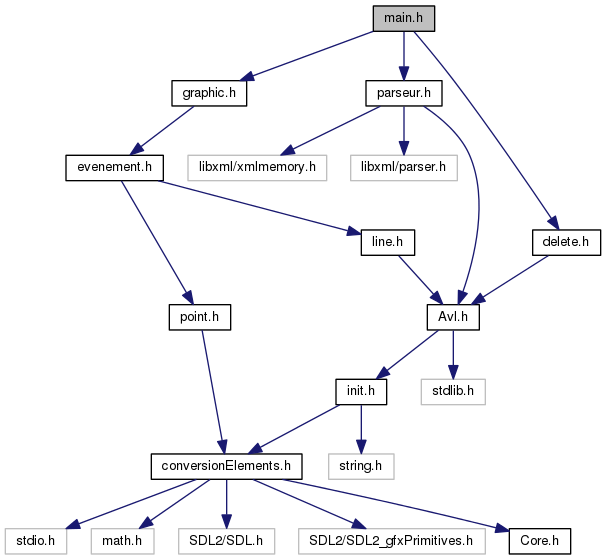
\includegraphics[width=7.9cm]{dependances.png}
	\end{center}
\end{frame}

\section{Graphe des fonctions}
\begin{frame}{Graphe des fonctions}
	\begin{center}
	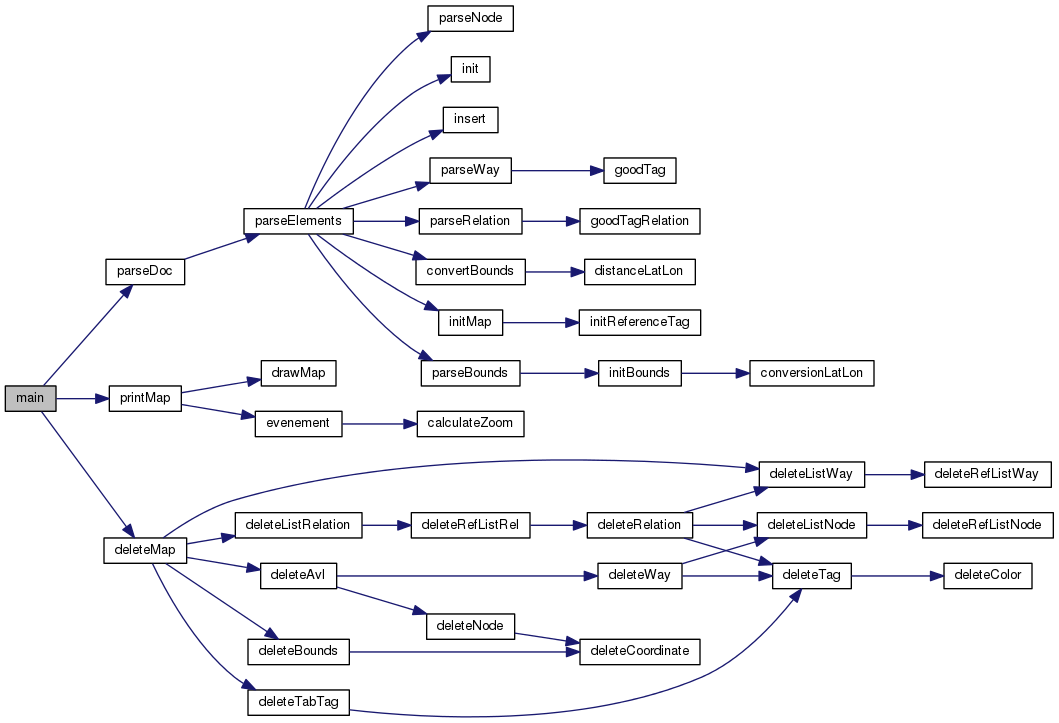
\includegraphics[width=10cm]{fonctions.png}
	\end{center}
\end{frame}

\section{Ordre de dessin}
\begin{frame}{Ordre de dessin}
	 \textbf{6 listes et une liste de relation}
	 \begin{itemize}
	 \item<2-8> \textbf{Water} (Rivage, rivière, ...)
 	 \item<3-8> \textbf{Relation} (Outer/Inner)
	 \item<4-8> \textbf{Green} (forêt, parc, espace vert, ...)
	 \item<5-8> \textbf{Other} (église, marina, pont) 
	 \item<6-8> \textbf{Building}
	 \item<7-8> \textbf{Highway} 
	 \item<8>     \textbf{Cadastre} (sources)

	\end{itemize}
\end{frame}

\section{Notre projet}
\begin{frame}{Notre projet}
	 \begin{itemize}
	 \item<1-5> \textbf{Projection}
 	 \item<2-5> \textbf{Relation} (Outer/Inner)
	 \item<3-5> \textbf{Zoom et déplacement} (à la souris et au clavier)
	 \item<4-5> \textbf{Coastline}
	 \item<5>	\textbf{Adaptation de la taille de la fenêtre en fonction des bounds }
	\end{itemize}
\end{frame}

\section{Doc, Check et performance}
\begin{frame}{Documentation, Check et performance}
  \begin{itemize}
	\item <1-9>\textbf{Documentation}
	\begin{itemize}
	\item  <2-9>Doxygen
	\end{itemize}
 	\item <3-9> \textbf{Check}
	\begin{itemize}
	\item  <4-9>tests\_unitaires
	\item  <5-9>cas limites
	\item  <6-9>check\_main
	\item  <7-9>Makefile
	\end{itemize}
	\item <8-9> \textbf{Test de performance}
	\begin{itemize}
	\item  <9>script de performance
	\end{itemize}
      \end{itemize}
\end{frame}

\section{Où nous en sommes}
\begin{frame}{Où nous en sommes}
	 \textbf{A améliorer}
	 \begin{itemize}
	 \item<1-3>\textbf{Nom des rues} (rotation)
	 \item<2-3>\textbf{Affichage nom des hotels, cafes} (taille, police de l'ecriture)
 	 \item<3> \textbf{Highway} (traçage en polygône)
	\end{itemize}
\end{frame}




\end{document}

